\documentclass[twoside]{wiss}

%\usepackage{ascmac}

\usepackage{graphicx}
\usepackage{here} % [H]とするとその場所に配置されるらしい

\long\def\EP{\textsf{EpisoPass}}
\long\def\PW{パスワード}
\long\def\SS{シード文字列}
\long\def\EM{エピソード記憶}

\journalhead{{\EP}: Holy Grail}

\begin{document}

\title{{\EP}: {\EM}にもとづく{\PW}生成}
%\etitle{{\EP}: The Ultimate Passwords Management System}
\etitle{{\EP}: Password Management based on Episodic Memories}

\author{増井俊之\affil{Toshiyuki Masui, 慶應義塾大学 環境情報学部}}

\begin{abstract}
忘却しにくい{\EM}にもとづく秘密の質問を使って強力な{\PW}を生成/管理するシステム「\textsf{\EP}」を提案する。
{\EP}は、ユーザの作成した秘密の質問への回答にもとづいて{\SS}を換字することによって強力な{\PW}を生成する。
{\SS}や回答のバリエーションにより異なる{\PW}が生成されるので様々なサービスに対して異なる{\PW}を生成できる。

秘密の質問の数が充分であれば、
あらゆる情報を公開しても強力な{\PW}を生成して利用することができる。
\end{abstract}

\maketitle

\section{はじめに}

個人認証のために{\PW}が現在広く利用されている。
{\PW}認証には多くの問題があることが知られているが\cite{増井_ユニマガ}、
今後も長期にわたって利用され続けることが予想されるため、
適切に運用するための工夫が必要になっている。

{\PW}の長期的記憶が難しいことは{\PW}認証の大きな問題点のひとつである。
安全に運用するためには{\PW}はランダムで長い文字列であることが望ましいが、
そのようなものを頭の中に記憶しておくことは難しい。
また複数のサービスを利用する場合、
サービスごとに異なる{\PW}を利用することが望ましいが、
すべての{\PW}を記憶しておくことはほとんど不可能である。
%
Flor\^{e}ncioの...における調査では...\cite{Florencio:2007:LSW:1242572.1242661}、
また2011年の野村総研の調査によれば、
一般的なユーザが{\PW}認証を行なうサイトは平均19.4個で、
利用している{\PW}は平均3.1個であった\cite{野村総研}。
多数の{\PW}を記憶することが困難であるため、
多くのユーザが同じ{\PW}を複数サイトで使い回しているのだと思われる。

異なる{\PW}をすべて記憶することは不可能なのでどこかに記録しておく必要があるが、
{\PW}をそのまま記録するのは危険なので、
複数の{\PW}を秘密情報として扱うための{\PW}管理システムが利用されている。
{\PW}管理システムは
1個の「マスター{\PW}」を利用してあらゆる{\PW}を管理するもので、
暗号化されたデータベースに{\PW}を格納するもの%
\cite{OnePassword}%
\cite{Dashlane}%
\cite{ミルパス}%
\cite{LastPass}%
\cite{KeyPass}%
\cite{NortonIDSafe}%
\cite{IDManager}%
が多いが、マスター{\PW}をサービス名で変換することによって
複数の{\PW}を生成するシステム\cite{SuperGenPass}もある。
% 前者はデータベースを解読される危険があるのに対し、
% 後者は{\PW}本体をどこにも保存していないためより安全であるが、
両者ともにマスター{\PW}の記憶は必須であり、
マスター{\PW}を盗まれたり忘れたりする危険がある。
% {\PW}を毎日使わない人なら忘れてしまう可能性は高い。

ユーザは{\PW}を忘れてしまうことが非常に多いため、
多くのサービスにおいて{\PW}を復元したり初期化したりする手段が用意されている。
ユーザが秘密の質問に対する答を登録し、
質問に正しく回答することによって{\PW}を復元したりリセットできるものがある。
また、秘密の質問に答えることによって
{\PW}管理システムのマスター{\PW}を復元するシステム\cite{平野亮:2011-11-07}も提案されている。

新しく覚えた情報や新しく考えた情報はどうしても忘れてしまう可能性があるので、
新しく作成した{\PW}文字列を記憶して認証に利用することは本質的に無理がある。
一方、既知で忘れることがない{\EM}を秘密の質問として
認証のために直接利用することができれば、
認証に必要な情報を忘れてしまうことがないはずである。
多くの画像認証システム\cite{小池英樹:2006-05-15}は
秘密の質問に対して正答を示すことによって認証を行なっているため
{\PW}のようなものを記憶する必要がない。
%認証方法を忘れにくいという特長がある。
% 秘密の質問が{\PW}と同じぐらい強力であれば、
% それをメインの認証手段にしてしまえばいいことになる。
%
画像認証システムはまだ普及していないためどこでも利用することができないが、
忘れない{\EM}を利用した秘密の質問への回答を強力な{\PW}に変換するシステムがあれば、
通常の{\PW}認証を用いた現在の様々なサービス上で{\PW}を忘れる心配なく安全な認証ができるようになる。
本論文ではこのようなシステム「{\EP}」について述べる。

\section{{\EP}}

\subsection{{\EP}の原理}

{\EP}は、
ユーザが忘れることがない個人的な{\EM}を文字列に変換することによって
安全な{\PW}を生成するシステムである。
{\PW}文字列は以下の手順で生成される。

\begin{enumerate}
\item {\PW}生成の「種」となる文字列を用意する。
以下ではこれを「{\SS}」と表現する。
\item 忘れることがない個人的な{\EM}にもとづく秘密の質問を複数作成し、
それぞれについてひとつの正答と複数の偽答を用意する。
\item 質問と回答の組にもとづいて{\SS}に換字操作を行なう。
すべてに正しく回答したとき生成される文字列を{\PW}として利用する。
\end{enumerate}

\subsection{{\EP}利用例}

以下に{\EP}の利用例を示す。

\paragraph{ブラウザでの利用}

筆者がtwitterの{\PW}を生成するために
ブラウザで{\EP}を利用している例を図\ref{web1}に示す\footnote{
  \textsf{http://{\EP}.com/masui}
}。
{\SS}として「\textsf{Twitter123456}」という文字列を指定しており、
4個の秘密の質問に対する回答選択に応じて
「\textsf{Mfveabn574923}」のような{\PW}候補が生成される。
{\SS}の8文字目が数字である場合は{\PW}の8文字目も数字になるなど、
{\SS}の文字種に対応した{\PW}候補が生成される。
最初の秘密の質問は筆者の小学校の同級生に関するもので、
最後の質問は数年前の体験に関するものである。
これらの質問は古い{\EM}にもとづいており、
筆者が将来答を忘れることはほとんど考えられないが、
本人以外がこのような質問に答えることは難しいので
他人が正しい{\PW}を得ることできない。

\begin{figure}[H]
\centerline{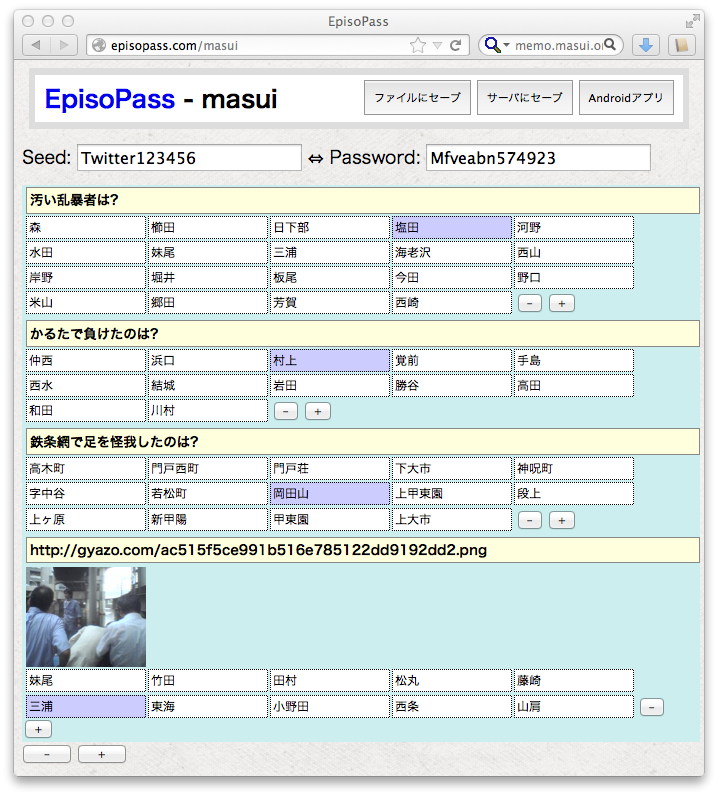
\includegraphics[width=83mm,bb=0 0 718 796]{figures/785ff09b4233804d2ec89c3af71ee5d0.png}}
\caption{ブラウザ上でTwitterの{\PW}を計算.}
\label{web1}
\end{figure}

秘密の質問と答はブラウザで編集でき、
「サーバにセーブ」ボタンを押すことにより{\SS}、秘密の問題、答のリストがサーバにセーブされる。
「ファイルにセーブ」ボタンを押すとJSONデータをパソコンにダウンロードでき、
JSONデータをブラウザにドラッグ\&ドロップするとサーバにアップロードできる。
ユーザはどれが正答かを指定しないので{\PW}がサーバに漏れる心配は無い。

{\SS}を「\textsf{Facebook123456}」に変更すると、生成される{\PW}は図\ref{web2}のようにが変化する。
このように、サービスごとに異なる{\SS}を利用することによって
様々な{\PW}を簡単に生成できる。

\begin{figure}[H]
\centerline{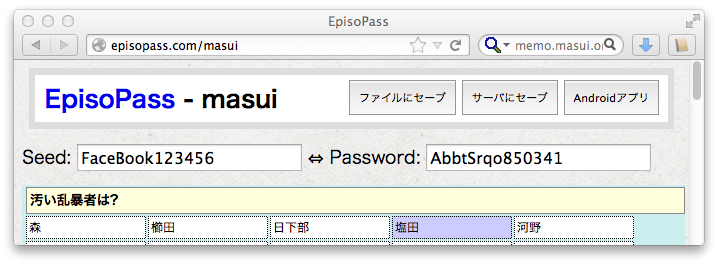
\includegraphics[width=83mm,bb=0 0 718 265]{figures/36c371a13a8250c60fb9c03174382443.png}}
\caption{FaceBookの{\PW}を計算.}
\label{web2}
\end{figure}

\paragraph{回答によりパスワードを変化}

サービスごとに{\SS}を変えるのではなく、
図\ref{web3}のように
サービス名に応じて回答を変えることによって異なる{\PW}を作成することも可能である。
{\PW}としての長さや文字種に特種な制約が無いサービスに関してはこの方法が便利である。

\begin{figure}[H]
\centerline{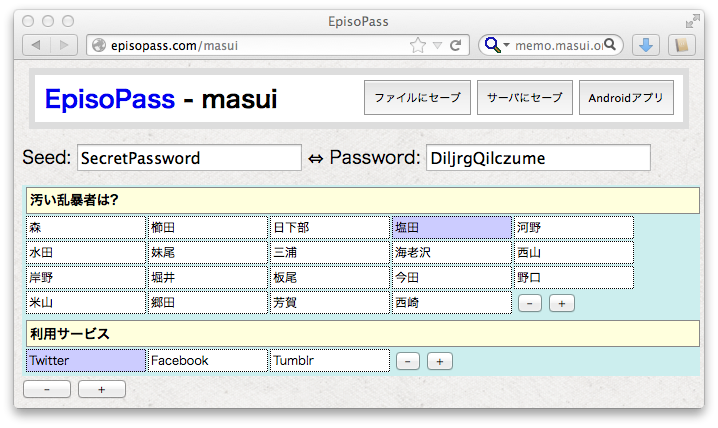
\includegraphics[width=83mm,bb=0 0 718 428]{figures/a9167a6ec6af9c70dd1617e3fc25ec30.png}}
\centerline{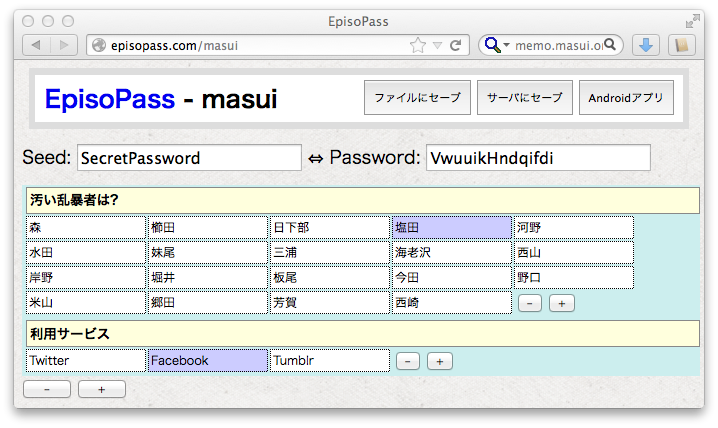
\includegraphics[width=83mm,bb=0 0 718 428]{figures/5b887fabeb8e3319623901fe4a6c56f2.png}}
\caption{サービス名に対応する回答で異なる{\PW}を生成.}
\label{web3}
\end{figure}

\paragraph{既存{\PW}の利用}

現在利用している{\PW}(e.g. ``\textsf{Masui1234}'')を利用したい場合、
図\ref{web4}のように{\PW}欄に現在の{\PW}を入力すれば
それを生成する{\SS}が自動生成されるので、
生成された{\SS}を記録しておけばよい。

\begin{figure}[H]
\centerline{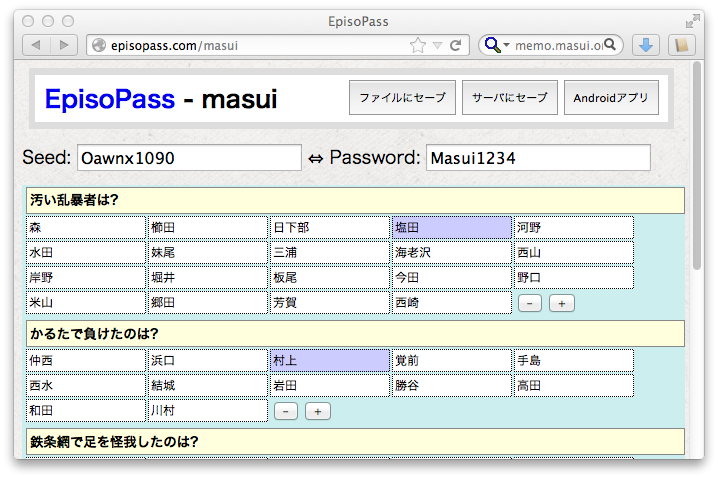
\includegraphics[width=83mm,bb=0 0 718 479]{figures/fab9c55242e1d52c89ff1b46d77b3168.png}}
\caption{既存の{\PW}を利用.}
\label{web4}
\end{figure}

{\PW}以外の秘密の文字列も管理することができる。
自転車の鍵番号「\textsf{1234}」を{\EP}で管理したい場合、
「\textsf{jitensha-0000}」という{\SS}を入力した後で
{\PW}枠の数字を「\textsf{1234}」に変更することにより、
図\ref{web5}のように「\textsf{jitensha-6145}」という{\SS}で
鍵番号を管理できるようになる。

\begin{figure}[H]
\centerline{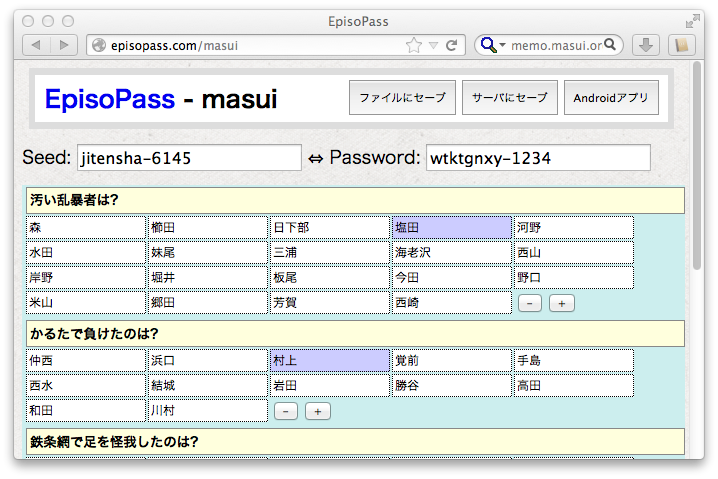
\includegraphics[width=83mm,bb=0 0 718 479]{figures/494cef6da1be0a069ee56e7ec8dcb9a7.png}}
\caption{既存の{\PW}を利用.}
\label{web5}
\end{figure}

\paragraph{Androidアプリ}

Webサービスを利用する場合、ブラウザとサーバとの間の通信を
記録されたり盗み見されたりされる危険が皆無ではない。
前述の例において、
{\PW}はブラウザ内部でJavaScriptにより生成されるので、
一度ページを表示した後は
ネットワークを遮断しても{\PW}計算を行なえるようになっているが、
最初から全く通信を行なわずに{\PW}を作成できる方がより安心であろう。
このため、通信を全く行なわずにマシン単体で{\PW}計算を行なうための
Androidアプリを用意した。
ブラウザの右上の「Androidアプリ」ボタンを押すと、
現在表示している秘密の問題と答を内蔵したAndroidアプリが
サーバ上でビルドされてダウンロード可能になる。

Android端末でアプリを実行すると図\ref{android1}のような画面が表示される。
{\SS}を設定して「開始」ボタンを押すと図\ref{android2}のように質問がひとつずつ表示され、
すべて回答すると{\PW}が計算され図\ref{android3}のように表示される。

\begin{figure}[H]
\centerline{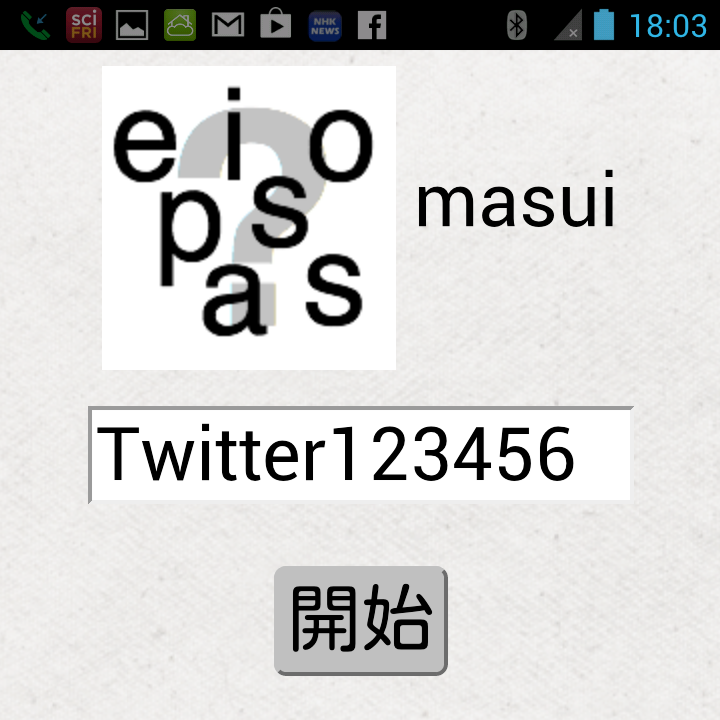
\includegraphics[width=50mm,bb=0 0 720 720]{figures/android1crop.png}}
\caption{Androidアプリ初期画面.}
\label{android1}
\end{figure}

\begin{figure}[H]
\centerline{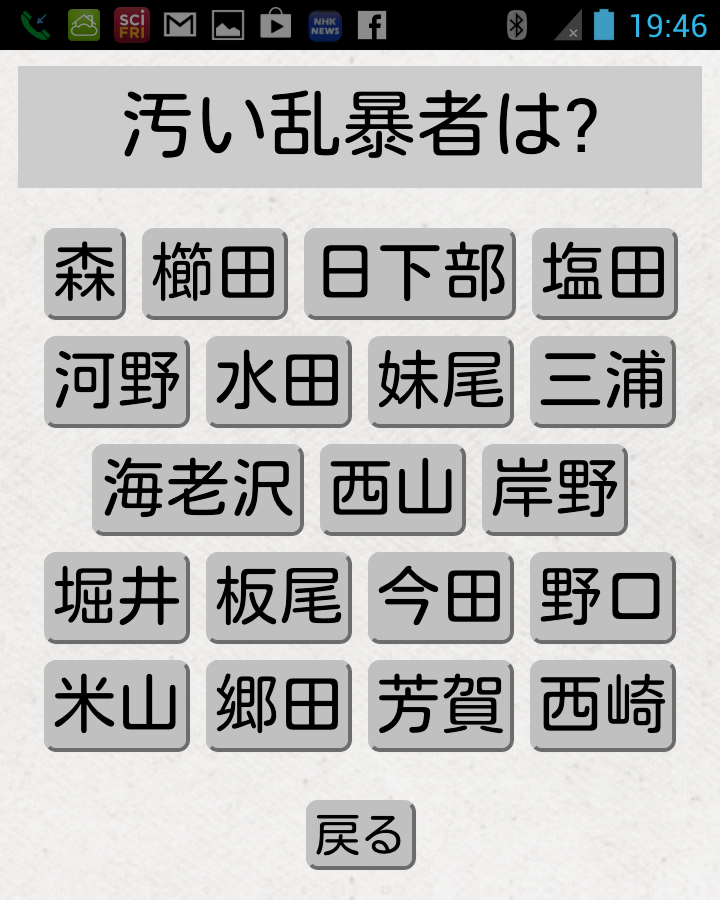
\includegraphics[width=50mm,bb=0 0 720 900]{figures/android2crop.png}}
\caption{最初の問題.}
\label{android2}
\end{figure}

\begin{figure}[H]
\centerline{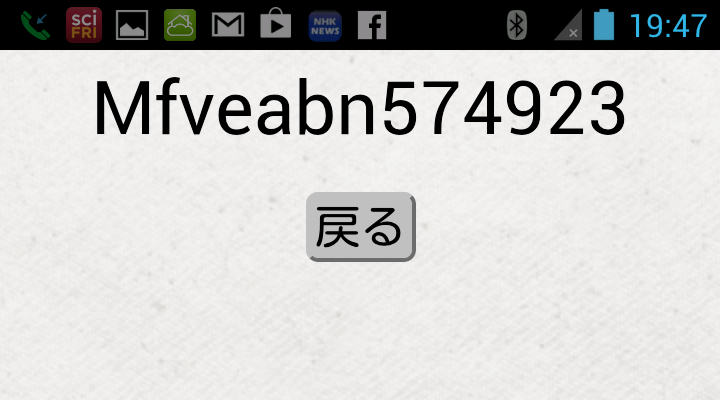
\includegraphics[width=50mm,bb=0 0 720 400]{figures/android3crop.png}}
\caption{すべての問題に回答した後の状態.}
\label{android3}
\end{figure}

回答入力と{\PW}計算はAndroid端末で実行されるため、
端末を「機内モード」に設定するなどの方法で
あらゆるネットワーク接続を遮断した状態でも{\PW}を計算することができる。
{\EP}をインストールしたAndroid端末を持っていれば常に各種の{\PW}を計算できるので、
他人のマシンや公共の場所に設置されたパソコンなどでも
安心してtwitterなどのネットサービスを利用することができる。

{\EP}アプリをサーバからダウンロードする場合は、
ブラウザ上で秘密の問題をサーバに登録する必要があるが、
秘密の問題を全くネット上に露出することなくアプリを利用することもできる。
秘密の問題を含まない{\EP}アプリをGoogle Playで公開しているので、
これを端末にインストールした後、
ローカルマシンで作成した秘密の質問を端末に転送すれば
EpisoPass.comからダウンロードしたアプリと同様に利用できる。
この手法を使うと秘密の質問がネット上に出現しないのでより安全であるが、
アプリのセットアップの手間は増える。

\subsection{{\PW}の計算方法}

問題と回答から文字列を生成し、そのMD5値によって{\SS}を換字することにより
{\PW}を生成している。

\section{議論}

\subsection{簡単か?}

原理は簡単で、ソースを全公開しているので
問題があれば指摘されることが期待できる

\subsection{{\PW}の生成と管理}

SuperGenPass\cite{SuperGenPass}は良いけれども
既存の{\PW}を登録することができない。

{\EP}は新しいものの生成も既存のものの記憶も両方できる

\subsection{画像の利用}

画像認証がイイと言ってる人も多い

画像も使えるよ

\subsection{他者が答を知っているときの危険}

自転車のカギ番号を共有しているとき
それを{\EP}で管理すると全質問の答がわかってしまう

家族のなぞなぞ問題を作るといった工夫

\subsection{運用レベル}

何を秘密にするかのレベルがある

\paragraph{\protect{\textsf{1. {\EP}}}の利用を秘密にする}

これは相当安全なはず。
{\EP}はあらゆる文字列を生成できるから。

\paragraph{\protect{\textsf{2.}} {\SS}を秘密にする}

SuperGenPassと同じレベル。
秘密の問題としてサービス名を使えば良い。

\paragraph{\protect{\textsf{3.}} すべて公開する}

秘密に記憶するものがひとつもないのでこれが一番楽ちん
実はこれでも大丈夫。
すべての計算結果を他人に見せなければ総当たり攻撃は回避できる。

\subsection{{\EM}をいろんなものに変換する面白さ}

{\PW}に限らないだろう

\subsection{指紋を{\PW}に変換することなども考えられる}

指紋はコピーされる

脳はコピーされない

同じ考え方は通用するだろう

\subsection{安全性}

エントロピー

\subsection{秘密の質問の脆弱性}

秘密の質問を解くことによって{\PW}をリセットできる機能があれば
{\PW}を忘れても大丈夫だという利点はあるものの、
このような方式がシステムを脆弱にしていることが近年問題になっている\footnote{
  ..... どこかの記者
}。

簡単な質問でリセットできるのが問題になっている。

秘密の質問は実は忘れることが多いという問題があるらしい。

平野\cite{平野亮:2011-11-07}は
秘密の質問からマスター{\PW}を復元する方法を提案している。
Shamirのなんたら方式を使い、全部正解しなくても復元できるのがミソ。

{\PW}は自分で考えることを想定しているのかもしれない?

% \textbf{どれが正解か知っていなければこの方法は適用できないのでは?}

{\EP}は、
{\PW}を忘れたときに秘密の質問を利用するのではなく、
{\PW}の生成に秘密の質問を利用するという点が異なっている。

兼子は、
秘密の質問のエントロピを上げる方法を提案している\cite{Kaneko}。

多くのシステムにおいて、
「母親の旧姓は?」や「最初に飼ったペットの名前は?」のような、
あらかじめ決まった質問のみを利用できるようになっているが、
このような問題は他人が解くことも容易であるうえに、
秘密の質問の数は少ないのが普通だからである\cite{Rabkin:2008:PKQ:1408664.1408667}。
% 銀行20個調べて秘密の質問の弱さを指摘

{\EP}はシステムに用意された問題を利用せず、
ユーザが自分で考えたなぞなぞ問題を利用するので、
他人には解くことが難しく自分では忘れない問題を自由に作成できる。
これは強力なはずであるが、
そのような問題を作成することは難しいということが
知られている\cite{Just:2009:PCC:1572532.1572543}\cite{Schechter:2009:NSM:1607723.1608145}。
%
%  秘密の質問の問題
%   自分で[[秘密の質問]]を決めるととても弱くなることが判明
%   複数の秘密の質問を使うとマシになる?
%   結構人は間違うものらしい
%  applicability or repeatability の問題がある
%   Applicability: How widely applicable is the given question?
%   Memorability: How easy is it for the user to recall the answer?
%   Repeatability: How accurately can the answer be replayed, without syntactic or semantic ambiguity?
%  ユーザに質問を作らせると全然駄目なことが多い
%   すぐ解けてしまうもの
%   思い出せないもの
%
% 自分が作るものでくだらない秘密の質問は駄目
%
古い記憶にもとづいて作成した秘密の問題はユーザが想像するよりも解かれやすい。
この問題を避けるため、問題と答を連想するために画像を利用したり、
複数の問題を連続的に利用したりする手法も提案されている\cite{Renaud:2010:PQE:2146303.2146318}。

%  昔の記憶にもとづく[[秘密の質問]]はアタックされやすい
%  質問に写真を加えることにより思い出しやすくなったり
%  解決策
%   答を思い出すために画像を使う
%    動物や場所の写真から人を思い出すなど
%   必ずしも本当でない連想を使う
%   連続的に出題する

% 秘密の質問はシステムに指定される場合とユーザが作成できる場合がある。
% システムが質問を提供する場合、あらゆるユーザが答えられる質問にしなければならないため、
% 「ペットの名前は?」「母親の旧姓は?」
% のような簡単なものであることが多いが、
% このような質問は他人が解くことも容易であるうえに、
% 質問の数も充分でないことが多いため充分安全でない\cite{Rabkin:2008:PKQ:1408664.1408667}。
% %
% ユーザが質問を作成できる場合、
% 他人に解くことが難しく自分では忘れない問題を自由に作成できるはずであるが、
% そのような問題を作成することは難しいということが
% 知られている\cite{Just:2009:PCC:1572532.1572543}\cite{Schechter:2009:NSM:1607723.1608145}。

\bibliographystyle{jwiss}
\bibliography{paper}

\end{document}
